\documentclass[a4paper, 11pt]{report}
\usepackage{epsfig}
\usepackage{graphics}
\usepackage{multirow}
\usepackage{multicol}
\usepackage{fancyhdr}
\usepackage{lastpage}
\usepackage{latexsym}
\usepackage[hang, scriptsize, bf]{caption}

\usepackage[utf8]{inputenc}

\usepackage{enumerate}

\usepackage{tikz}
\usepackage[european]{circuitikz}

\usepackage{stackengine}
\usepackage{scalerel}
\usepackage{xcolor}


\usepackage{tikz-qtree}
\usetikzlibrary{arrows,shapes,snakes,positioning,automata}
\usetikzlibrary{shapes.multipart}
\usetikzlibrary{patterns,shapes}


\usepackage{wasysym}

\usepackage{algorithmic}
\usepackage{listings}

\usepackage{multirow}
\usepackage{multicol}

\usepackage{hhline}
\usepackage{array}
\usepackage{longtable}

\newcommand\dangersign[1][2ex]{%
  \renewcommand\stacktype{L}%
  \scaleto{\stackon[1.3pt]{\color{red}$\triangle$}{\tiny\bfseries !}}{#1}%
}
%-------------------------------------------------------------------------------

\textwidth      170mm
\textheight     240mm
\hoffset        -10mm 
\voffset        -10mm
\oddsidemargin   5mm
\evensidemargin -5mm
\topmargin	    -5mm

%-------------------------------------------------------------------------------

\newcommand{\eduTitle}{Zadání laboratoře}
\newcommand{\eduID}{4}
\newcommand{\eduTopic}{Polovodičové součástky -- dioda, tranzistor}
\newcommand{\eduDetails}{
\footnotesize
Cíle: 
Experimentálně ověřit chování 
polovodičových součástek 
ve vybraných praktických obvodových zapojeních.
}
%
\newcommand{\subjIDlong}{Elektronika pro informační technologie}
\newcommand{\schoolDlong}{Vysoké učení technické v Brně}
\newcommand{\schoolDshort}{VUT v Brně}
\newcommand{\facultylDlong}{Fakulta informačních technologií}
\newcommand{\facultylDshort}{FIT}
%
\newcommand{\subjIDshort}{IEL}
%
\newcommand{\actYear}{2024}
\newcommand{\acadYear}{2024/2025}

\usepackage[hidelinks]{hyperref}

\renewcommand{\figurename}{Obrázek}

%-------------------------------------------------------------------------------

\newcommand*\circled[1]{\tikz[baseline=(char.base)]{
            \node[shape=circle,draw,inner sep=2pt] (char) {#1};}}

%-------------------------------------------------------------------------------

\newcounter{cntInfo}
\newcommand{\info}[3]{\refstepcounter{cntInfo}
\paragraph*{
\circled{\thecntInfo}~{\sc \fbox{#1}} {\sc #2}  
}  
\paragraph{\textmd{#3}} }

%-------------------------------------------------------------------------------

\begin{document}

%-------------------------------------------------------------------------------

\pagestyle{fancy}
\renewcommand{\headrulewidth}{0pt}

\renewcommand{\theenumi}{\Alph{enumi}} 
\lhead{}
\chead{}
\rhead{}
\lfoot{\centering
\tiny \itshape \eduTitle ~č. \eduID \hspace{0.1mm} z předmětu \subjIDshort \hspace{1mm} 
(ak. r. \acadYear). \copyright~\actYear~Josef~Strnadel,~\facultylDshort~\schoolDshort. Připomínky zasílejte na \href{mailto:strnadel@fit.vut.cz}{strnadel@fit.vut.cz}\\ 
Časové razítko PDF dokumentu [\pdfcreationdate]. 
Sazba byla provedena systémem \LaTeX.
 }
\cfoot{}
%-------------------------------------------------------------------------------

%-------------------------------------------------------------------------------

\begin{center}
\scalebox{0.1}{
\includegraphics{FIT_cernobile_CZ.pdf}}
\parbox{120mm}{
\textsc{\footnotesize\schoolDlong}, 
\textsc{\footnotesize\facultylDlong}\\
}
{
\Large
\textsc{\subjIDlong} (\textsc{\subjIDshort}), \textsc{ak. r. \acadYear}}

\hrulefill

\vspace{4mm}
\parbox{\linewidth}{
\centering
%
{\Huge \textsc{\eduTitle~č.~\fbox{\eduID}}}\\
{\textsc{,,\eduTopic''}}\\

}

\end{center}

{\it \eduDetails}

\hrulefill

%-------------------------------------------------------------------------------
\vspace{-2mm}
\info{Motivace}{aneb ,,Proč tomu věnovat čas a jaké kompetence lze získat ?''\vspace{-3mm}}{
Na základě sady experimentů budete moci ověřit, pochopit a objasnit 
princip 
činnosti 
vybraných obvodových zapojení s polovodičovou diodou a 
tranzistorem, a 
související děje a jevy\protect\footnote{mj. diodový jev, tranzistorový jev}. 
Např. získáte zkušenost s propustným a závěrným směrem diody 
a bipolárním tranzistorem\protect\footnote{typu n-p-n (npn, NPN) v zapojení se společným emitorem (SE)}
ve funkci spínače\protect\footnote{od tranzistorového spínače se mj. očekává: dva stavy (sepnuto, rozepnuto), malá spotřeba výkonu, krátká doba a~vysoký opakovací kmitočet spínání/rozepínání}.
}

%-------------------------------------------------------------------------------
\info{Výstup a způsob jeho hodnocení}{aneb ,,Co se ode mne očekává a co za to ?''\vspace{-3mm}}{
Za experimentální ověření činnosti obvodů s polovodičovými součástkami, dějů v nich probíhajících,
souvisejících jevů  
a objasnění jejich využití v praxi 
lze získat až {\bf 3 body}.
}


\def\CalcC#1{%
\coordinate (base) at (#1.B);
\coordinate (collector) at (#1.C);
\coordinate (emitter) at (#1.E);
\draw (barycentric cs:base=0.32,collector=0.5,emitter=0.5) circle [radius=14pt];
}


%-------------------------------------------------------------------------------
\info{Prostředky}{aneb ,,Co je k dispozici ?''\vspace{-3mm}}{
~
}

Zdroj ss. napětí s omezením proudu,
nepájivé pole, 
krabička s prvky pro konstrukci obvodů (rezistory, dioda, tranzistor, vodiče), 
měřicí přístroje (multimetr, osciloskop).
\\

\vspace{-4mm}

\begin{figure}[h!]
\centering
\parbox{15mm}{
\vspace{-12mm}
\scalebox{0.5}{
    \begin{circuitikz}
\draw (0,0) node[twoportshape,t=N](boxK){};
\draw (0,1.0) node[twoportshape,t=P](boxA){};
\draw (boxK.south) to (0,-.85) node[below] {Katoda ({\bf K})};
\draw (boxA.north) to (0,1.85) node[above] {Anoda ({\bf A})};
            \end{circuitikz}
}}
\parbox{10mm}{
\vspace{-12mm}
\scalebox{0.85}{
    \begin{circuitikz}
      \draw (0,0)
      to[diode, l_={}, i_={}] (0,-1.5);
	\node at(.25,0) {A};
	\node at(.25,-1.5) {K};
    \end{circuitikz}
}
}\hspace{4mm}
\parbox{10mm}{
\vspace{-12mm}
\scalebox{0.25}{
	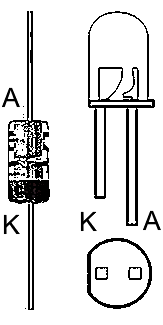
\includegraphics[trim={0mm 0mm 0mm 0mm},clip]{led-package3.png}
}
}
\hspace{4mm}
\parbox{10mm}{
\vspace{-12mm}
\scalebox{0.85}{
    \begin{circuitikz}
      \draw (0,0)
      to[led, l_={}, i_={}] (0,-1.5);
	\node at(-.25,0) {A};
	\node at(-.25,-1.5) {K};
    \end{circuitikz}
}}
\hspace{20mm}
\scalebox{0.08}{
	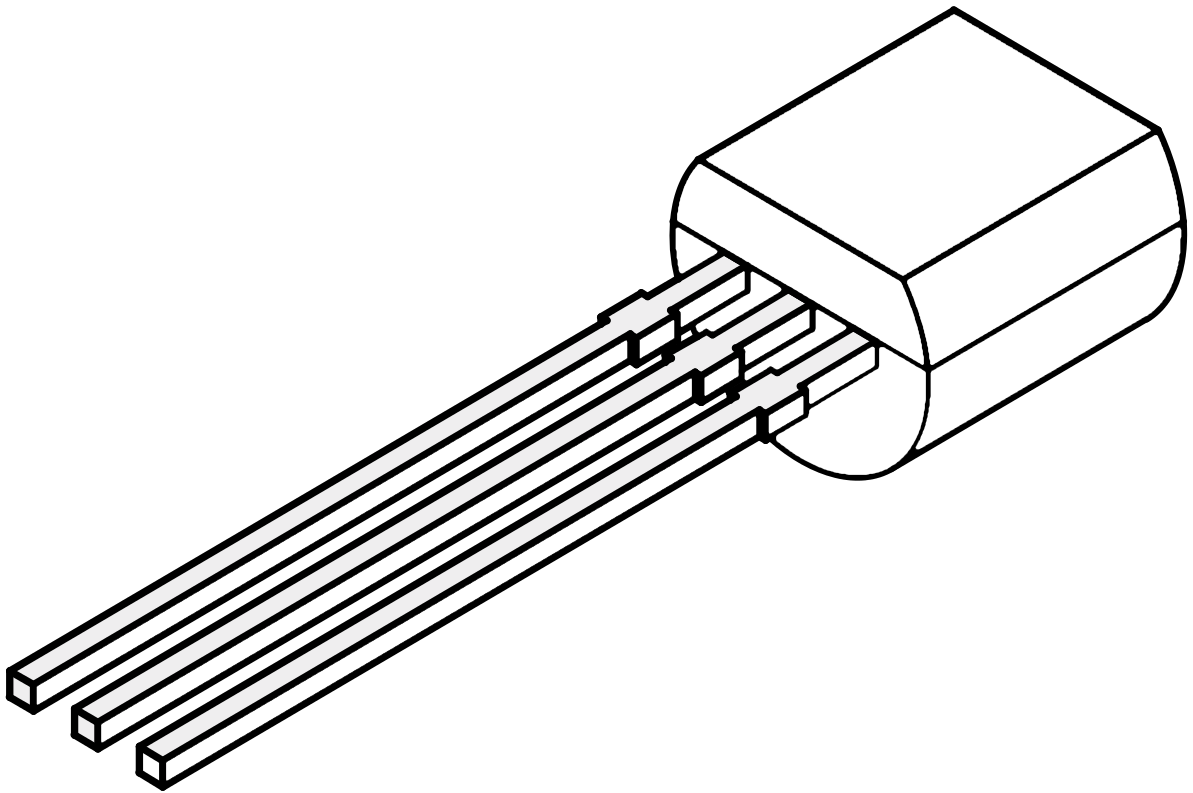
\includegraphics[trim={0mm 0mm 0mm 0mm},clip]{TO-92.png}
}
%
%
%
\hspace{-32mm}
%
%
%
\parbox{30mm}{
\vspace{3mm}
\footnotesize
\begin{circuitikz}
\node at(0,-.1) {C};
\node at(.25,-.3) {B};
\node at(.5,-.5) {E};
\end{circuitikz}
}
\scalebox{.9}{
\parbox{20mm}{
\vspace{-10mm}
\begin{circuitikz} 
\draw (0,0) node[npn] (name) {}
(name.base) node[anchor=east] {B}
(name.collector) node[anchor=south] {C}
(name.emitter) node[anchor=north] {E};
\CalcC{name}
\end{circuitikz}
}}
\parbox{10mm}{
\vspace{-10mm}
\scalebox{0.5}{
    \begin{circuitikz}
\draw (0,0) node[twoportshape,t=N](boxE){};
\draw (0,1.0) node[twoportshape,t=P](boxB){};
\draw (0,2.0) node[twoportshape,t=N](boxC){};
\draw (boxE.south) to (0,-.85) node[below] {Emitor ({\bf E})};
\draw (boxB.east) to (1,1) node[right] {Báze ({\bf B})};
\draw (boxC.north) to (0,2.85) node[above] {Kolektor ({\bf C})};
            \end{circuitikz}
}}

\vspace{-3mm}
   \caption{Vývody, průřez materiálem, značka a pouzdro a) polovodičové diody, b) bipolárního NPN tranzistoru;
   povšimněte si, že zatímco v diodě je jediný PN přechod, v bipolárním tranzistoru jsou PN přechody dva.} % typu n-p-n.}
   \label{fig_led1}
   \vspace{-4mm}
\end{figure}



%-------------------------------------------------------------------------------
\info{\vspace{-2mm}Základní schéma(ta)}{aneb ,,Z čeho se bude vycházet ?''\vspace{-2mm}}{
~
}

\vspace{-6mm}
\begin{figure}[h!]
  \begin{center}

\scalebox{0.95}{
\parbox{60mm}{
\vspace{-40mm}
%
    \begin{circuitikz}
      \draw (0,0)
      to[american voltage source,invert,v<=5~V, i^={}] (0,1.5) % The voltage source
     to[R,  l_=$R$, i^={}] (3,1.5)
      to[led, color=red, l_=$D$, i_={}] (3,0) % The resistor
      to[short] (0,0);
\draw node at (-2.0,0.75) {a)};
     \draw(2,-0.5) node {~};
    \end{circuitikz}
\\
  \begin{circuitikz}
      \draw (0,0)
      to[american voltage source,invert,v<=5~V, i_={}] (0,1.5) % The voltage source
     to[R,  l_=$R$, i^={}] (3,1.5)
      to[led, color=red, invert, l_=$D$, i^={}] (3,0) % The resistor
      to[short] (0,0);
\draw node at (-2.0,0.75) {b)};
     \draw(2,-0.5) node {~};
    \end{circuitikz}
}}
\hspace{4mm}
\scalebox{.85}{
\begin{circuitikz} \draw
(0,0) node[npn] (npn) {}
(npn.base) node[anchor=south, color=black] {\bf B}
(npn.collector) node[anchor=north west, color=black] {\bf C}
(npn.emitter) node[anchor=west, color=black] {\bf E};

\draw(-4,0) node[left] {1} to [R,  l_=$R_B$, i_=\textcolor{red}{$I_B$}, o-] (npn.base);
\draw (4.5,2.5)  node[right] {} to[led, l^=$D$, i_=\textcolor{red}{$I_C$}, mirror, -] (0,2.5) to [R,  l^=$R_C$, i_={}] (npn.collector);
\draw(npn.collector) to [short, *-o] (2,0.770) node[right] {2};
\draw(npn.emitter) to [short, i_=\textcolor{red}{$I_E$}] (0,-1.5) to (0,-1.5) node (gnd) [ground] {};

\draw (4.0,2.25) edge  [->, bend left=30, line width=.25, color=gray] node[above = 10mm]{\hspace{0mm}$U_{CC}$} (2.0,-1.25);
\draw (2.0,0.5) edge  [->, bend left=25, line width=.25, color=gray] node[right = 3mm]{\parbox{4mm}{\vspace{-6mm}$U_{2}$}} (0.5,-1.25);
\draw (-3.75,-0.25) edge  [->, bend left=-30, line width=.25, color=gray] node[left=8mm]{\parbox{4mm}{\vspace{-6mm}$U_{1}$}} (-0.5,-1.75);

\draw (4.5,2.5) to[american voltage source,v>=5~V, i_={}] (4.5,-1.5) node {} to[short, -*] (gnd) node {};

\draw (npn.collector) + (.45,-0.5) edge  [->, bend left=30, color=blue] node[right]{$U_{CE}$} (.25,-.5);
\draw (npn.collector) + (-.35,0.0) edge  [->, bend left=-40, color=blue] node[left = 2mm]{$U_{CB}$} (-1.25,.25);
\draw (npn.base) + (-.2,-0.4) edge  [->, bend left=-30, color=blue] node[left]{$U_{BE}$} (-.25,-0.85);

\draw (-2.0,2) node {\parbox{4cm}{
\textcolor{blue}{$U_{CE} = U_{CB} + U_{BE}$}\\
\textcolor{red}{$I_{E} = I_{C} + I_{B}$}
}};
%
\draw node at (-5.0,-1.5) {\scalebox{1.18}{c)}};
\draw[dashed, color=gray] (-2.25,-.5) ellipse (2.5cm and 1.25cm) node[above left=8mm]{
\rotatebox{0}{
\parbox{10mm}{\centering spínací\\část}
}
};
\draw[dashed, color=gray] (0.75,.5) ellipse (1.0cm and 2.0cm) node[above right=4mm]{
\rotatebox{0}{
\hspace{-5mm}
\parbox{15mm}{\centering spínaná\\část}
}
};

\CalcC{name}
\end{circuitikz}
}

\vspace{-4mm}
   \caption{Obvod s diodou a) v propustném resp. b) v závěrném směru,
   c) spínač s bipol. NPN tranzistorem v~zapojení SE; promyslete okolnosti, za kterých jsou resp. mohou být některé z PN přechodů v tranzistoru zapojeném dle c) v~propustném či závěrném směru.} 
   \label{fig_schema}
  \end{center}
\vspace{-6mm}
\end{figure}



%-------------------------------------------------------------------------------
\info{Postup samostatných činností}{aneb ,,Co dělat a na co si dát pozor ?''}{
~
}



\vspace{-6mm}


\begin{enumerate}[\bf {Experiment} 1:]

\item 
V nepájivém poli zapojte obvod dle Obr. \ref{fig_schema}a; 
poté
odměřte napětí na součástkách 
a sledujte, zda a za jakých podmínek dioda svítí\footnote{svítící dioda signalizuje průchod nezanedbatelného proudu obvodem}.
Činnosti opakujte pro Obr. \ref{fig_schema}b.
{\bf Objasněte} souvislost zjištěného chování diody s tzv. \emph{diodovým jevem}\footnote{závislost elektrického odporu diody na polaritě a velikosti vnějšího napětí přiloženého na diodu}.

\item 
\begin{enumerate}[i)]
\item
V nepájivém poli zapojte obvod dle Obr. \ref{fig_schema}c; 
zapojení obohaťte o potenciometr pro regulaci hodnoty napětí $U_1$
v rozmezí $0~V$ až $5~V$.

\item
Odměřte závislost chování tranzistorového spínače z Obr. \ref{fig_schema}c
na hodnotě napětí $U_1$. 
Do sloupců tab. z Obr. \ref{fig:tab_char}a 
doplňte 
chybějící údaje pro $U_1$ z jejího záhlaví.

\item Na základě tabulky z Obr. \ref{fig:tab_char}a vyneste grafy závislosti $U_2$=$f$($U_1$) a $U_{BE}$=$g$($U_1$).
{\bf Objasněte} souvislost zjištěných závislostí s tzv. \emph{tranzistorovým jevem}\footnote{malé napětí vzbuzuje v obvodu báze proud, který je příčinou vzniku mnohem většího proudu v kolektorovém obvodu}
a
ozna- čování tranzistorového spínače pojmem \emph{invertor logické úrovně}\footnote{měnící log.0 na log.1 a naopak; např., log.0 si lze představit jako napětí pod $0,4~V$, log.1 jako napětí nad $0,6~V$}.

\item 
{\bf Předveďte} činnost tranzistoru ve funkci spínače, 
{\bf určete} 
pracovní body 
tranzistorového spínače
pro stavy sepnuto, rozepnuto
a
{\bf objasněte} pohyb mezi těmito pracovními body\footnote{např. ve Výstupní charakteristice  tranzistoru (graf závislosti $I_C$ a $U_{CE}$) -- viz přednášky aj.}. 

\end{enumerate}



\vspace{-4mm}
\begin{figure}[h]
\centering
\hspace{4mm}
\parbox{2mm}{
\footnotesize
\vspace{-24mm}
\hspace{-4mm}
a) 
}
\hspace{-12mm}
\parbox{85mm}{
\centering
\scalebox{.85}{
\begin{tabular}{|c||c|c|c|c|c|c|c|c||c|}
\hline
\bf $U_1$ &~~0~~&0,3&0,5&0,6&0,8&~~1~~&~~3~~&~~5~~&\multirow{3}{*}{[V]}\\
\cline{1-9}
\bf $U_{BE}$ &&&&&&&&&\\
\cline{1-9}
\bf $U_{2}$ &&&&&&&&&\\
\hline
Svit LED &&&&&&&&& [\%]\\
\hline
\end{tabular}
}
}
\hspace{22mm}
\parbox{2mm}{
\footnotesize
\vspace{-16mm}
b) 
}
\hspace{-16mm}
\parbox{70mm}{
\centering
\scalebox{.85}{
\begin{circuitikz} 
\draw (0,0) node[npn] (npn) {};

\draw(-2.5,0) node[left] {\bf B} to [R,  l_=$R_B$, o-] (npn.base);
\draw (0,2.5)  node[left,, color=red] {$U_{CC}$ = +5~V} to [R,  l_=$R_C$, o-] (npn.collector);
\draw(npn.emitter) to [short] (0,-0.5) to (0,-0.5) node[ground] {};

\draw (-4.0,0) node[npn] (npn2) {};
\draw(-6.5,0) node[left] {\bf A} to [R,  l_=$R_A$, o-] (npn2.base);
\draw(npn2.emitter) to [short] (-4,-0.5) to (-4,-0.5) node[ground] {};

\draw (npn2.collector) to [short, -*] (npn.collector);
\draw (npn.collector) to [short, -o] (1,.77) node[right] {\bf C};

\draw (-6.5,-0.25) edge  [->, bend left=-30, line width=.25, color=gray] node[left=5mm]{$U_{A}$} (-5.0,-1.0);
\draw (-2.5,-0.25) edge  [->, bend left=-30, line width=.25, color=gray] node[left=5mm]{$U_{B}$} (-0.5,-1.0);
\draw (1,.5) edge  [->, bend left=30, line width=.25, color=gray] node[right=0mm]{$U_{C}$} (0.5,-1.0);

\CalcC{npn2}
\CalcC{npn}

\end{circuitikz}
}
}
\vspace{-2mm}
   \caption{a) příklad tab. pro záznam výsledků experimentu 2, b) schéma obvodu k experimentu 3}
   \label{fig:tab_char}
\vspace{-2mm}
\end{figure}


\item

V rámci zvolené skupiny experimentálně ověřte, popř. pomocí dosud nabytých vědomostí
{\bf objasněte} princip činnosti obvodu z Obr. \ref{fig:tab_char}b (log. vstupy $A$, $B$ a log. výstup $C$; log.0 resp. log.1 realizujte připojením k $0~V$ resp. $5~V$)
a 
{\bf zjistěte}, 
kterou log. funkci realizuje;
nakreslete či zapojte {\bf jiný} log. obvod pomocí dvou tranzistorů.  


\end{enumerate}

%-------------------------------------------------------------------------------
\info{Shrnutí, vyhodnocení a interpretace výsledků}{aneb ,,Jaká jsou zjištění ?''\vspace{-2mm}}{
Experimentálně jste mohli ověřit
důsledky a praktické využití dvou jevů -- diodového, tranzistorového.
Mj. se podařilo zjistit, že za běžných okolností dioda propouští proud pouze v jednom směru, 
a to za cenu určitého  úbytku napětí na ní; 
toto chování 
lze využít v řadě aplikací\protect\footnote{např. ke konstrukci usměrňovačů či logických hradel, 
k ochraně prvků před následky napěťových špiček atd.}.
%
Dále jste mohli ověřit, že 
i)~od tranzistorového, stejně jako u mehanického, spínače se čekají pouze stavy sepnuto resp. rozepnuto,
mezi nimiž pracovní bod tranzistoru při spí/rozepínání přechází\protect\footnote{v případě odporové zátěže v kolektoru přechází po tzv. zatěžovací přímce}
ii) 
vstupně-výstupní chování tr. spínače je realizací invertoru log. úrovně a je základem dalších logických obvodů.
}

%-------------------------------------------------------------------------------
\info{K zamyšlení/zapamatování}{aneb ,,Něco do dalšího studia a života.''\vspace{-2mm}}{
Na základě získaných poznatků o chování diody 
zkuste 
navrhnout 
obvod, který je  
schopen převést vstupní střídavé napětí (či proud) na stejnosměrné,
popř. logické hradlo.
Zkuste zjistit, zda tr. spínač přechází mezi stavy sep/rozepnuto po přímce i v případě kapacitní či induktivní zátěže v kolektoru.
}




\end{document}
